
\section{Additional Experimental Results}
\subsection{Bayesian Neural Network Regression}\label{section:bnn_additional}

\begin{figure}[H]
  \centering
  \subfloat[Wine]{
    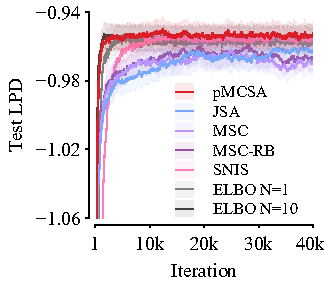
\includegraphics[scale=0.9]{figures/wine_01.pdf}
  }\hspace{0.2in}
  \subfloat[Wine]{
    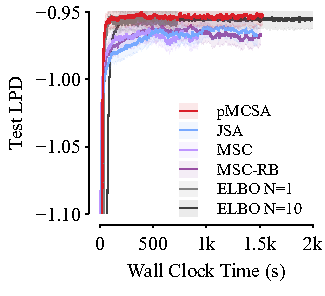
\includegraphics[scale=0.9]{figures/wine_02.pdf}
  } \\
  \subfloat[Concrete]{
    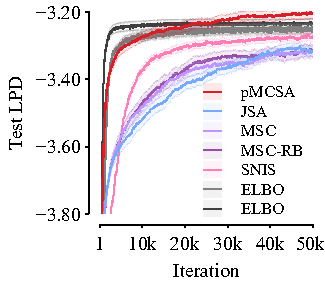
\includegraphics[scale=0.9]{figures/concrete_01.pdf}
  } \hspace{0.2in}
  \subfloat[Concrete]{
    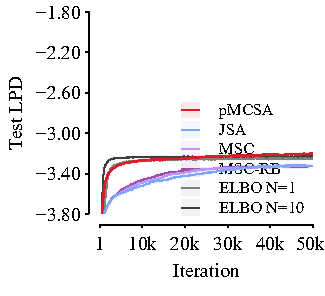
\includegraphics[scale=0.9]{figures/concrete_02.pdf}
  } \\
  \subfloat[Boston]{
    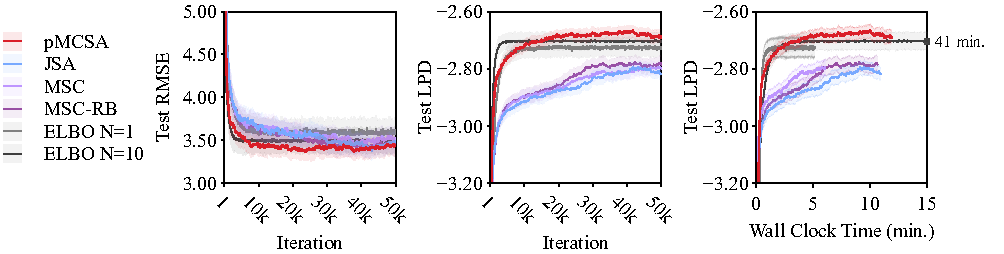
\includegraphics[scale=0.9]{figures/boston_01.pdf}
  }\hspace{0.2in}
  \subfloat[Boston]{
    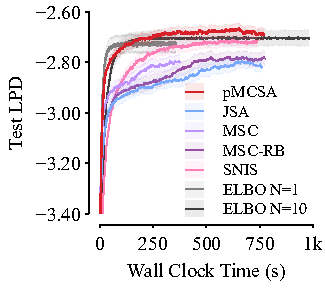
\includegraphics[scale=0.9]{figures/boston_02.pdf}
  } \\
  \subfloat[Yacht]{
    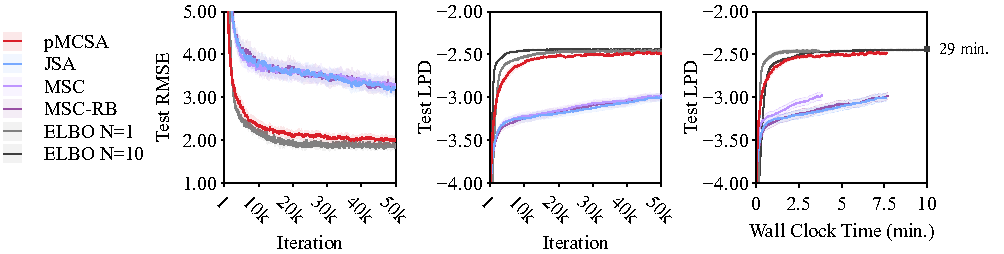
\includegraphics[scale=0.9]{figures/yacht_01.pdf}
  }\hspace{0.2in}
  \subfloat[Yacht]{
    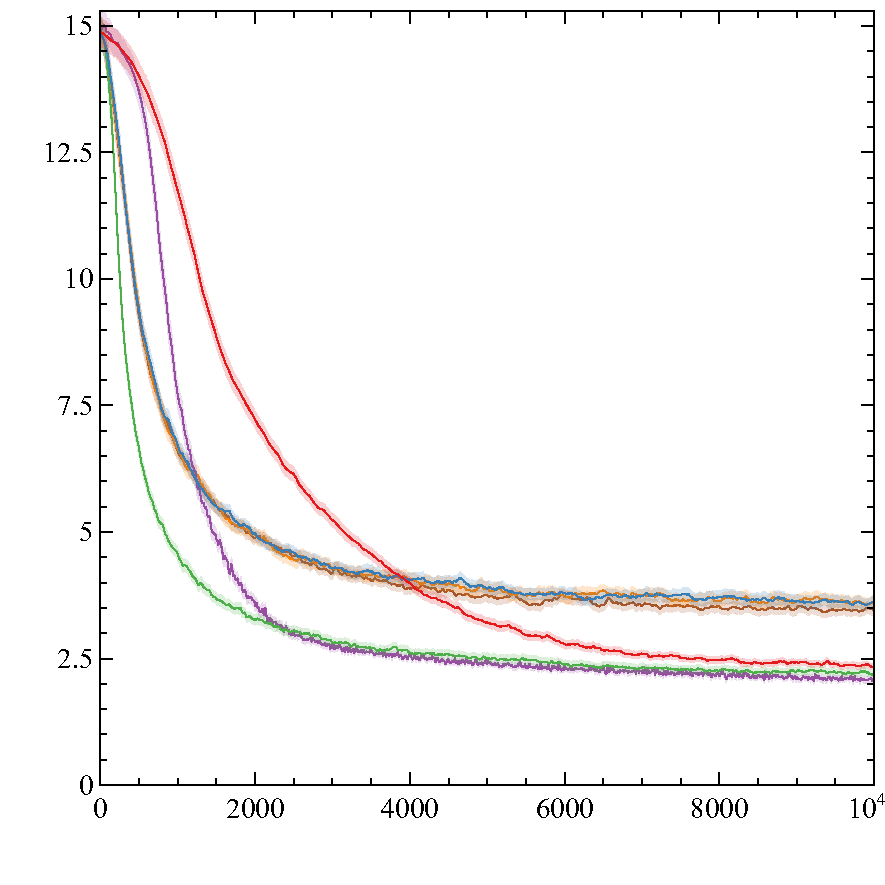
\includegraphics[scale=0.9]{figures/yacht_02.pdf}
  }
  \caption{Bayesian Neural Network Regression}
\end{figure}

\begin{figure}[H]
  \centering
  \subfloat[Airfoil]{
    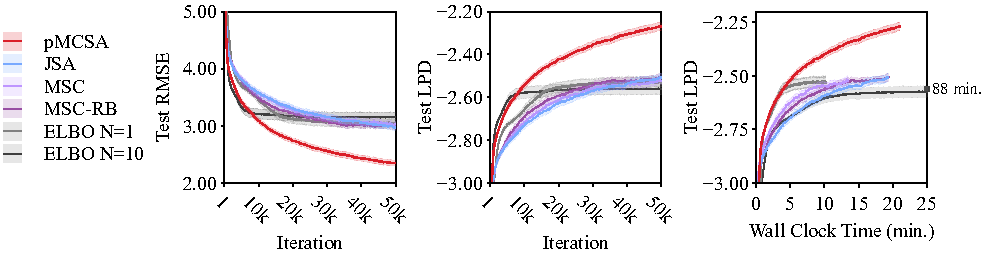
\includegraphics[scale=0.9]{figures/airfoil_01.pdf}
  }\hspace{0.2in}
  \subfloat[Airfoil]{
    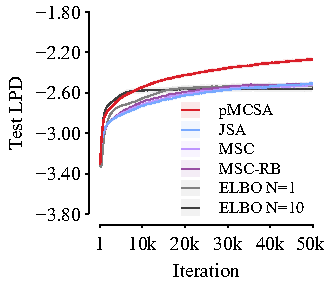
\includegraphics[scale=0.9]{figures/airfoil_02.pdf}
  } \\
  \subfloat[Gas]{
    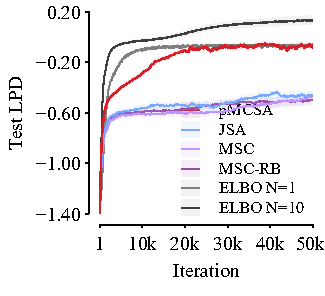
\includegraphics[scale=0.9]{figures/gas_01.pdf}
  } \hspace{0.2in}
  \subfloat[Gas]{
    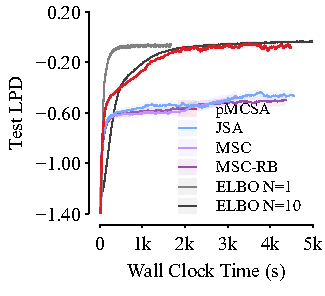
\includegraphics[scale=0.9]{figures/gas_02.pdf}
  } \\
  \subfloat[Energy]{
    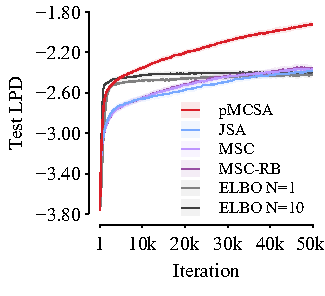
\includegraphics[scale=0.9]{figures/energy_01.pdf}
  }\hspace{0.2in}
  \subfloat[Energy]{
    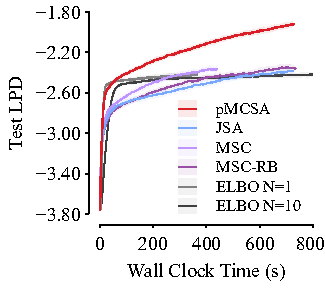
\includegraphics[scale=0.9]{figures/energy_02.pdf}
  } \\
  \subfloat[SML]{
    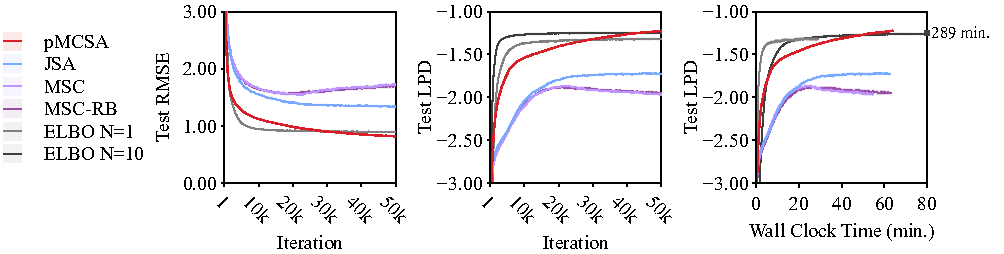
\includegraphics[scale=0.9]{figures/sml_01.pdf}
  }\hspace{0.2in}
  \subfloat[SML]{
    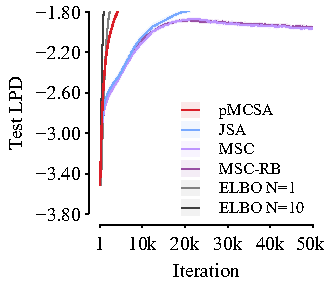
\includegraphics[scale=0.9]{figures/sml_02.pdf}
  }
  \caption{Bayesian Neural Network Regression}
\end{figure}

\subsection{Robust Gaussian Process Regression}\label{section:gp_additional}
\begin{figure}[H]
  \centering
  \subfloat[Wine]{
    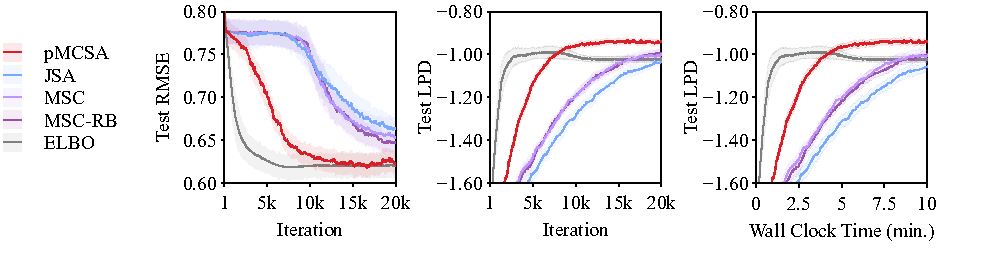
\includegraphics[scale=0.9]{figures/wine_pgp_01.pdf}
  }\hspace{0.2in}
  \subfloat[Wine]{
    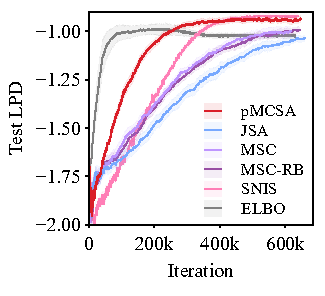
\includegraphics[scale=0.9]{figures/wine_pgp_02.pdf}
  } \\
  \subfloat[Concrete]{
    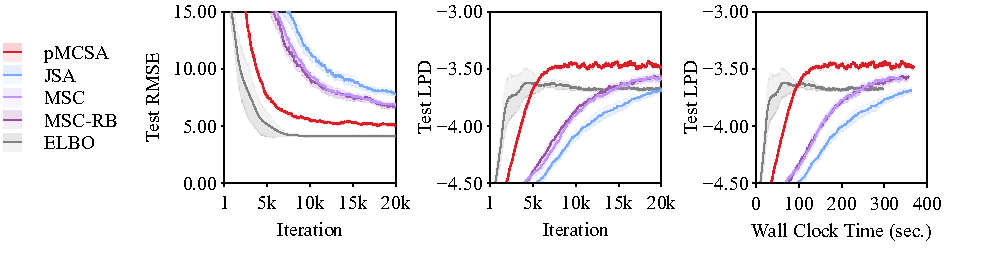
\includegraphics[scale=0.9]{figures/concrete_pgp_01.pdf}
  } \hspace{0.2in}
  \subfloat[Concrete]{
    \includegraphics[scale=0.9]{figures/concrete_pgp_02.pdf}
  } \\
  \subfloat[Boston]{
    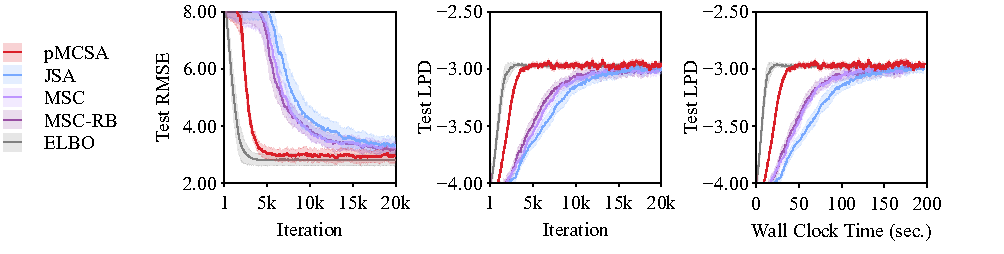
\includegraphics[scale=0.9]{figures/boston_pgp_01.pdf}
  } \hspace{0.2in}
  \subfloat[Boston]{
    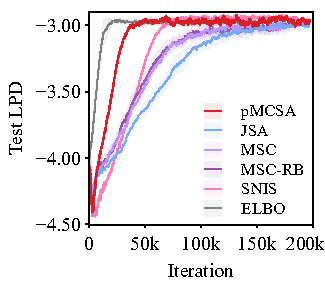
\includegraphics[scale=0.9]{figures/boston_pgp_02.pdf}
  } \\
  \subfloat[Yacht]{
    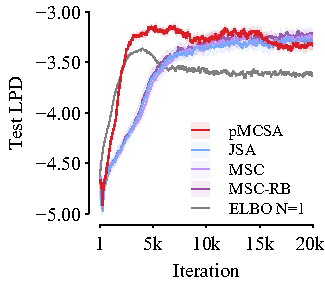
\includegraphics[scale=0.9]{figures/yacht_pgp_01.pdf}
  } \hspace{0.2in}
  \subfloat[Yacht]{
    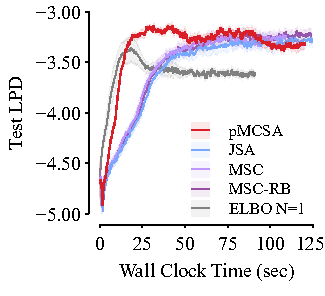
\includegraphics[scale=0.9]{figures/yacht_pgp_02.pdf}
  }  
  \caption{Robust Gaussian Process Regression}
\end{figure}

\begin{figure}[H]
  \subfloat[Airfoil]{
    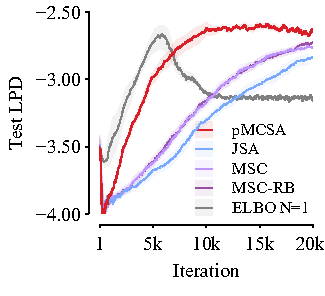
\includegraphics[scale=0.9]{figures/airfoil_pgp_01.pdf}
  } \hspace{0.2in}
  \subfloat[Airfoil]{
    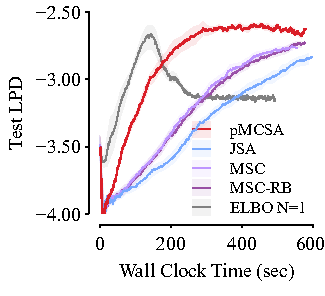
\includegraphics[scale=0.9]{figures/airfoil_pgp_02.pdf}
  } \\
  \subfloat[Energy]{
    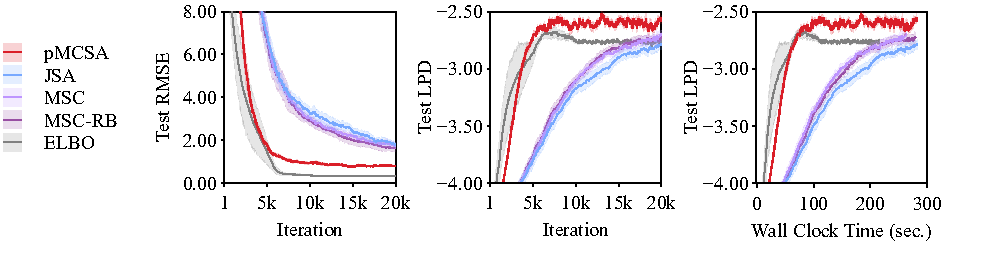
\includegraphics[scale=0.9]{figures/energy_pgp_01.pdf}
  } \hspace{0.2in}
  \subfloat[Energy]{
    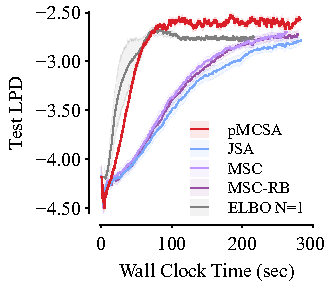
\includegraphics[scale=0.9]{figures/energy_pgp_02.pdf}
  } 
  \caption{Robust Gaussian Process Regression}
\end{figure}

%%% Local Variables:
%%% TeX-master: "master"
%%% End:
